\documentclass[12pt]{article}
\usepackage{times,amsmath,amsthm,amsfonts,graphicx,float,cite}
\usepackage{epstopdf,tikz,mathrsfs,dsfont,geometry,tabularx,booktabs}
\usepackage{pdflscape,tcolorbox}
\usepackage{clrscode3e}
\usepackage{enumerate}
\usepackage{mathtools}
\restylefloat{table}
\DeclarePairedDelimiter\ceil{\lceil}{\rceil}
\DeclarePairedDelimiter\floor{\lfloor}{\rfloor}
%===========================================
% Page Margins
\setlength{\oddsidemargin}{0in}
\setlength{\evensidemargin}{0in}
\setlength{\topmargin}{-0.5in}
\setlength{\textwidth}{6.5in}
\setlength{\textheight}{9in}
\setlength{\headsep}{0.25in}
\setlength{\parindent}{0in}
\setlength{\parskip}{0.05in}
%===========================================
% The following commands set up the num (number) counter and
% make various numbering schemes work relative to the problem number.
\newcounter{num}
\renewcommand{\thesection}{Problem~\arabic{section}}
%===========================================
% The following macro is used to generate the header.
\newcommand{\header}[3]{
\setcounter{num}{1}
\noindent
\begin{center}
\framebox{
\vbox{
\vspace{2mm}
\hbox to 6.28in { {Missouri University of Science \& Technology \hfill Department of Computer Science} }
\hbox to 6.28in { {\bf Fall 2018 \hfill CS 2300: Databases} }
\vspace{2mm}
\hbox to 6.28in { {\bf \large \hfill Solutions to Homework #1  \hfill} }
\vspace{2mm}
\hbox to 6.28in { {\bf Name: {\it #2} \hfill Email: {\it #3}} }% Scribe: {\it #3}} }
\vspace{2mm}
}
}
\end{center}
\vspace*{2mm}
}
%===========================================
% User-defined theorems, commands and other math operators
\newtheorem{defn}{Definition}
\newtheorem{thrm}{Theorem}
\DeclareMathOperator*{\modulo}{modulo}
%===========================================
%===========================================

% The main document begins here...
\begin{document}
% Define your header here
\header{1}{Andrew Henningsen, Evan Wilcox}{achcdp@mst.edu}
%===========================================
\section{}
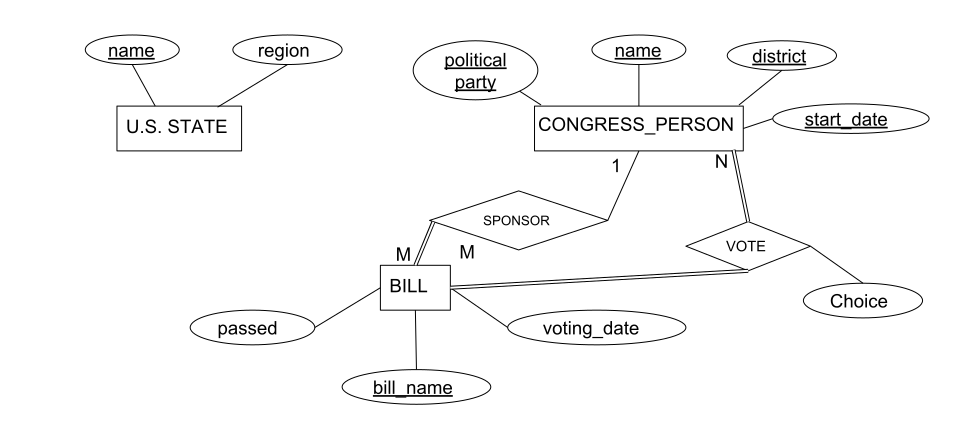
\includegraphics[scale=0.7]{Problem1}
Assumptions: \\
\begin{enumerate}
	\item We assume that the congress person's name cannot be uniquely identified by just name, district, and political party as people like George W Bush can have the same name, district, and political party but different start dates. 
    \item A congressperson will always vote on a bill but if they are absent or abstain it will be stored in their choice.
    \item A congress person can sponsor many bills but a bill will only have one sponsor.
\end{enumerate}
\newpage

%===========================================
\section{}

\begin{enumerate}
    \item Year, Semester, CRoom and DaysTime must be unique in order for only one section to use a particular classroom at a particular day and time. If section is included, this would imply that they can teach two sections at the same time of day.
    \item Instructor, Year, Semester, CRoom, and DaysTime must be unique in order for an instructor to only teach one section at a particular day and time. If section is included, this would imply that they can teach two sections at the same time of day.
    \item Office and phone number must be unique so that no two departments can share the same office and phone number. If Department is included, then they would be able to share a same office and phone number.
\end{enumerate}
\newpage
%===========================================
\section{}
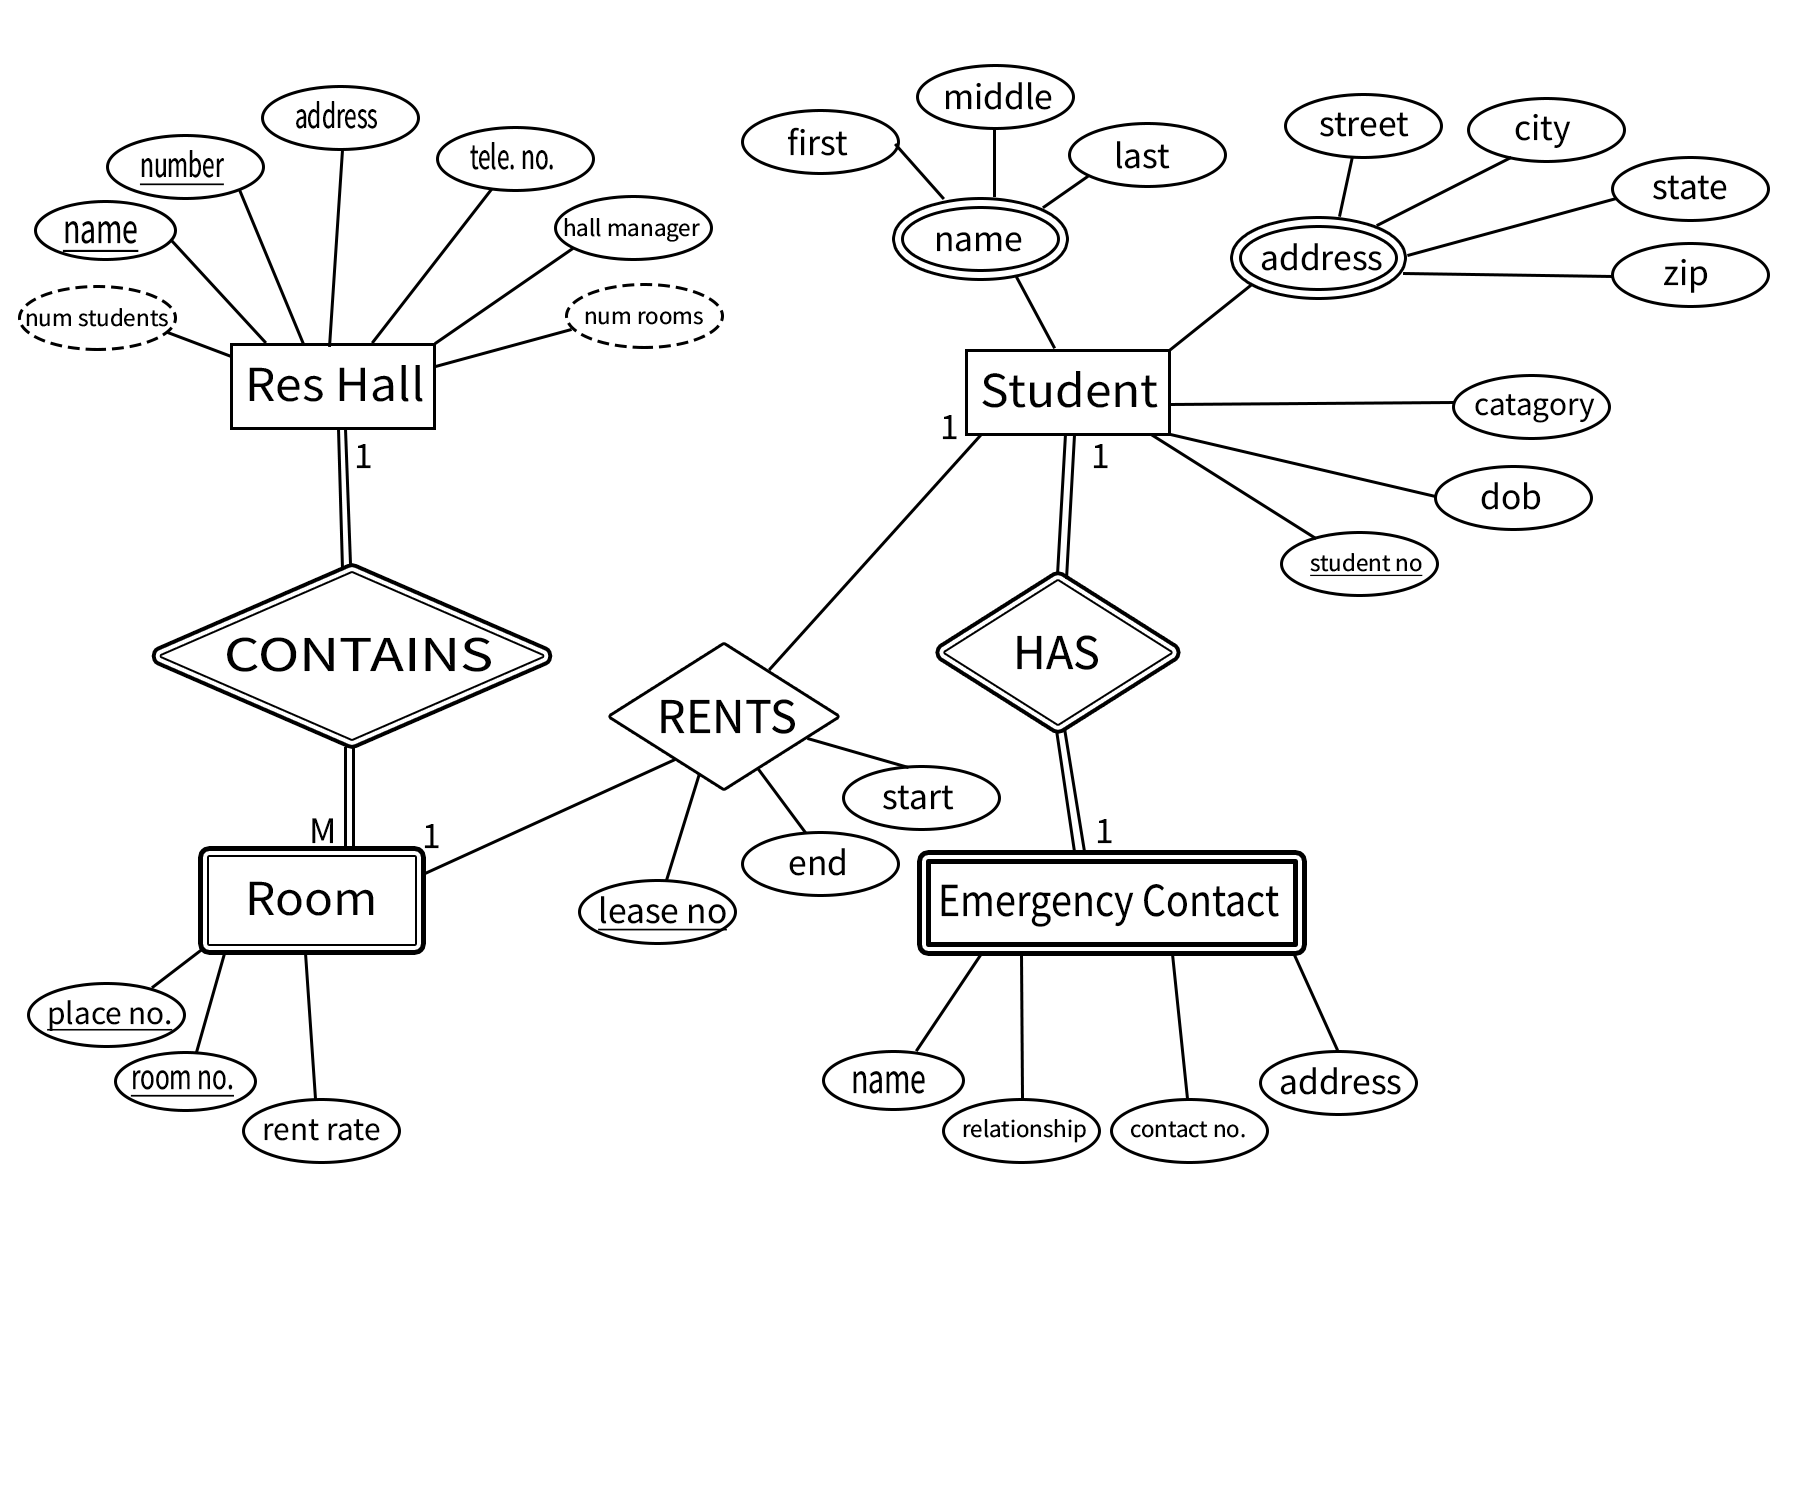
\includegraphics[scale=0.3]{Problem3.png}
\begin{enumerate}
    \item A student only has one emergency contact so the emergency contact can be uniquely identified by the relationship to a certain student.
    \item Multiple Res Halls can have the same name but will have a different number (RC1, RC2)
    \item A student cant rent multiple rooms
    \item A room can be empty/a student doesn't have to rent a room and may live off campus.
\end{enumerate}
\newpage
%===========================================
\section{}
\begin{enumerate}[a.]
    \item Track Capacity = Block Size * Number of Blocks per Track = 512 * 28 = 14,336 bytes.
    \item Cylinder Capacity = Track Capacity * Tracks per Surface = 14,336 * 500 = 7,168,000 bytes.
    \item Disk Pack Capacity = Cylinder Capacity * Num Disks = 7,168,000 * 8 * 2 = 114,688,000 bytes.
    \item 
    \begin{itemize}
        \item Transfer Rate = $\frac{\textrm{track size}}{\textrm{time to spin once}} =  \frac{14,336 * 60 * 1000}{2400}$ = 14,336 bytes/ms.
        \item Block Transfer Time = $\frac{\textrm{block size}}{\textrm{bytes transferred per ms}} = \frac{512}{358,400}$ = 0.00143ms.
        \item Rotational Delay = $\frac{1}{2} * \frac{60*1000}{2400}$ = 12.5ms.
    \end{itemize}
    \item (Seek Time + Rotational Delay + Block Transfer Time) = (30ms + 12.5ms + 0.00143ms) = 42.50143ms
    \item 
        \begin{itemize}
            \item Time for 20 random blocks = 850.028ms
            \item Time for 20 consecutive blocks = 250.029ms.
        \end{itemize}
\end{enumerate}
\newpage
\end{document}